\section{Future Work}
\label{sec:future}

\begin{sidewaysfigure}
  \centering
  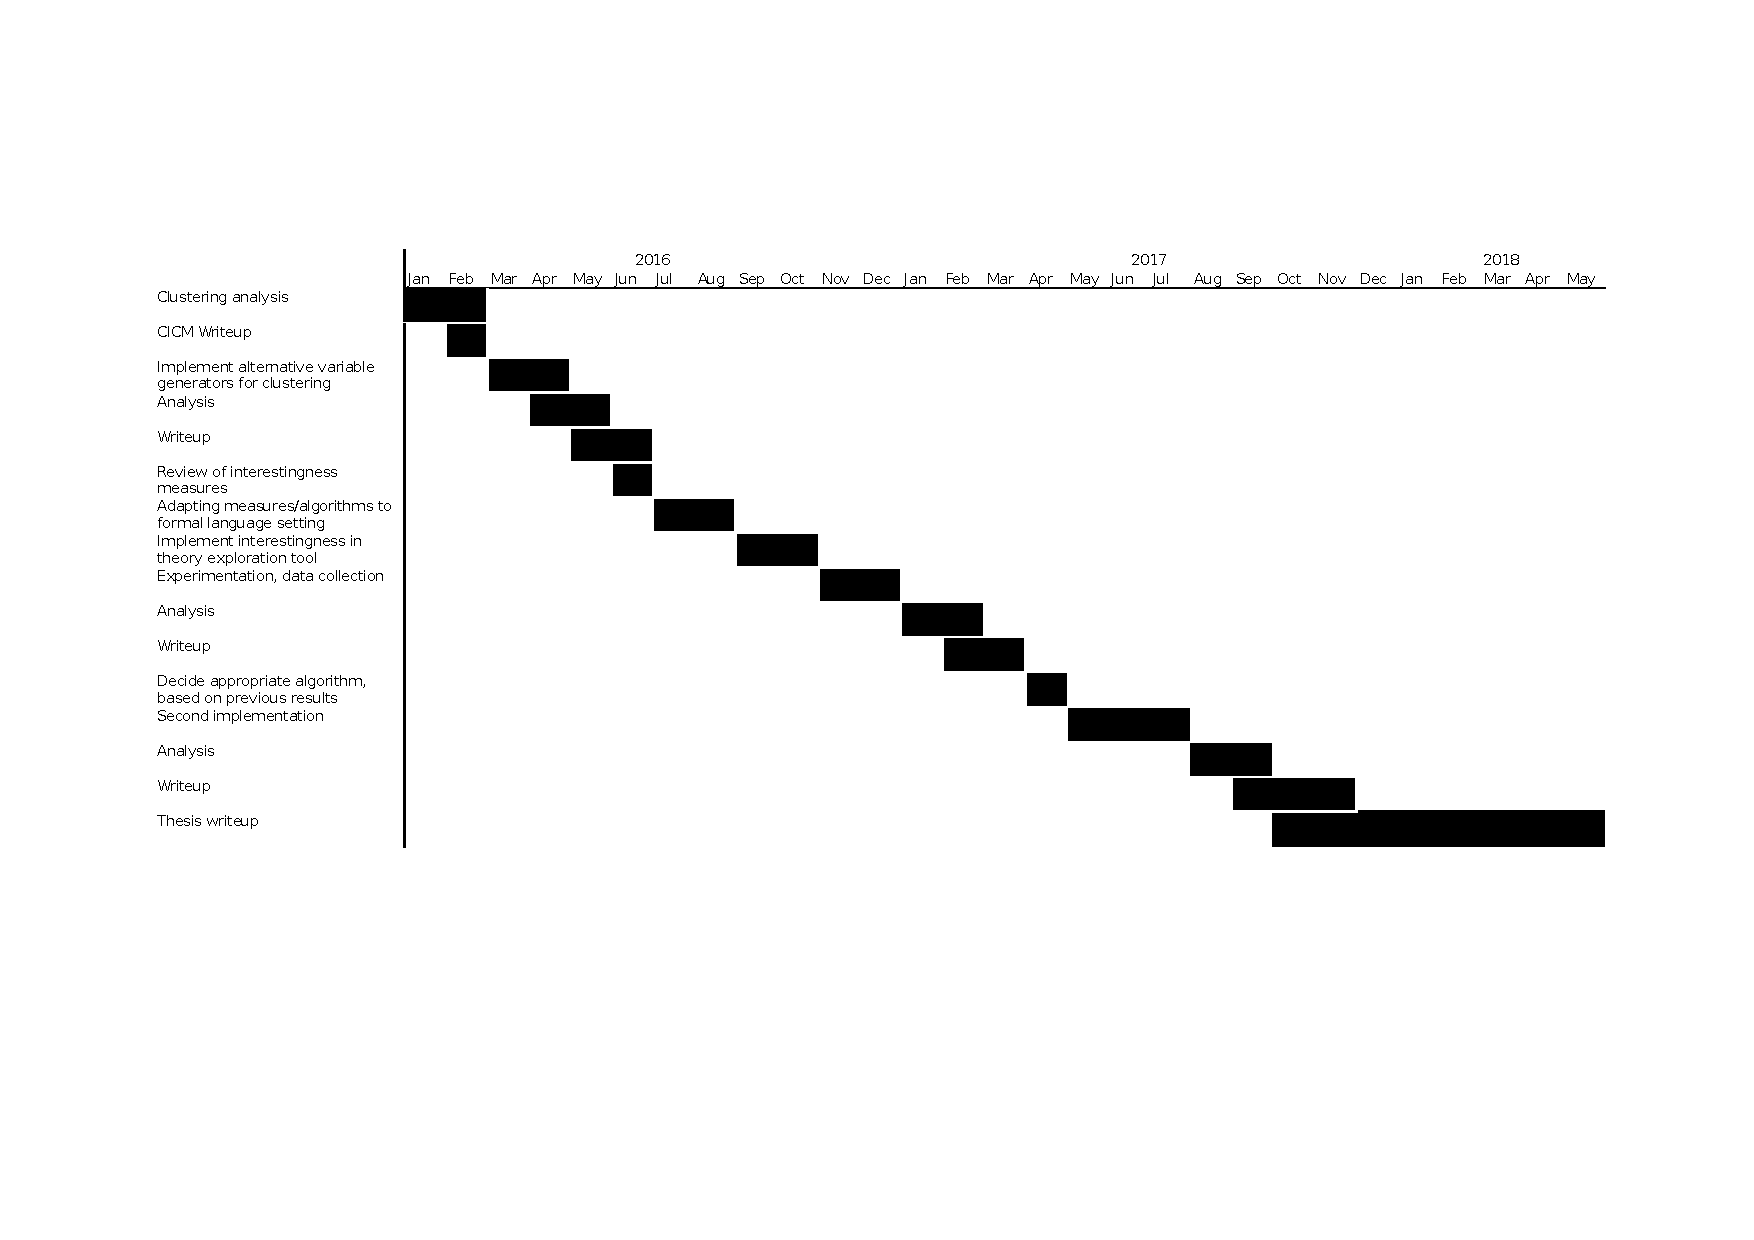
\includegraphics[trim=3cm 2cm 3cm 2cm, width=1.00\textwidth]{Gantt.pdf}
  \caption{Gantt chart showing research direction, sub-tasks and approximate timeframes. CICM is the \emph{Conference on Intelligent Computer Mathematics}.}
  \label{fig:gantt}
\end{sidewaysfigure}

Our use of clustering to pre-process \qspec{} signatures has required many decisions and tradeoffs to be made. Hence our approach is just one possibility out of many alternatives which could be investigated to push this work further. In addition, there are other ways in which machine learning could aid theory exploration besides our relevance filter technique. The Gantt chart in Figure \ref{fig:gantt} shows how these relate to the short- and long-term direction being taken by this research. Below, we elaborate on the details, background and motivation for these choices.

\subsection{Clustering Extensions}
\label{sec:preprocessing}

The most glaring omission in our algorithm is its disregard for types. By ignoring types, not only are we losing valuable information about expressions, but we also lose the ability to distinguish between constructors. This is because a constructor, like \hs{True} or \hs{Just}, has no internal structure; it is just a token. The distinguishing features of constructors are their types, which not only tell us which data type they construct, but also their arity, the types of their arguments, etc.

Our algorithm closely follows that of ML4PG, which \emph{does} support types. This is handled by populating matrix cells with tokens \emph{and} their types. Unfortunately this is more complicated in Haskell than it is in Coq, since types form a separate part of the language from terms, and we do not have an interactive Core environment to query for types (unlike ML4PG, which runs inside the Proof General environment).

One partial solution would be leave most Core expressions without types, but to include them for non-local identifiers (i.e. globals and constructors), which we can look up in a database. In fact, our ML4HS framework already includes such type information in its database, alongside the Core syntax trees. Integrating this information into our algorithm is the next logical step.

We can also compare the performance of our hand-selected features with \emph{learned} representations, like those reviewed in \citep{bengio2013representation}. This may provide an indication of how important it is to understand the language when identifying salient aspects of expressions, and how difficult various aspects of it might be to learn.

With more expressive features, it may also be useful to experiment with more powerful learning algorithms. An interesting possibility is to add a feedback loop between the theory exploration phase and the clustering phase, to more directly base the similarity of expressions on whether they (are predicted to) occur together in equations.

\subsection{Theory Exploration Extensions}

Our current approach is a rather conservative change to the existing theory exploration approaches, as it is essentially a wrapper around \qspec{}. There is potential for more radical changes to be made, which alter the search process itself.

\subsubsection{Variable Instantiation}

\qcheck{} is certainly the most popular property checker for Haskell, which motivates its use in \qspec{} to instantiate variables to random values. However, this task of finding type inhabitants has also been solved in many other ways, which may be worth investigating in place of \qcheck{} (or perhaps even as part of an ensemble).

The \textsc{SmallCheck} system \citep{runciman2008smallcheck} \emph{enumerates} values rather than sampling them randomly. Whilst this does not make \textsc{SmallCheck} objectively ``better'' than \qcheck{}, one major advantage is that it may use much less memory, as the generated values are built up incrementally. In contrast, \qcheck{} may generate very large values; in particular, generating tree structures na\"{\i}vely can cause them to grow exponentially. For example, here is a potential generator for \hs{RoseTree}s:

\begin{lstlisting}[language=Haskell, xleftmargin=0.1\textwidth, xrightmargin=0.1\textwidth]
genRoseTree = do f        <- arbitrary
                 subtrees <- listOf genRoseTree
                 return (Node f subtrees)
\end{lstlisting}

The \hs{listOf genRoseTree} call will return a list of arbitrary length, where each element is generated by \hs{genRoseTree}. This allows an arbitrary number of recursive calls to be made for each invocation of \hs{genRoseTree}, which will quickly exhaust the resources of any machine. Whilst such problems may be anticipated, or quickly spotted, in a property checking setting, this can be more difficult for our automated approach. For example, if a type does not have a generator available, we cannot use a library like \hs{derive} to create one automatically, as it suffers from this na\"{\i}vity problem.

A relative of \textsc{SmallCheck} is \textsc{Lazy SmallCheck} \citep{reich2013advances}, which uses laziness to only produce parts of a datastructure as they are demanded. This may narrow down our search procedures greatly, especially when predicates are involved. \qcheck{} allows predicates to restrict the values it tests with, and hence allows \emph{conditional} equations to be discovered. However, its implementation uses a simple rejection sampling technique: values are generated just as if the predicate were not there, and afterwards are filtered to reject any which do not satisfy the predicate. This makes it difficult to use very specific predicates, as it is unlikely that many of our random samples will exactly match our criteria. On the other hand, \textsc{Lazy SmallCheck} will focus its search on exactly those parts of the datastructure which are checked by the predicate, as those are the parts being forced to evaluate. This makes it much more likely that we will find values which satisfy the predicate, allowing us to effectively explore more specific conditional properties.

Other approaches to generating inhabitants include \textsc{Djinn} \citep{augustsson2005djinn}, which uses a decision procedure for a sub-set of Haskell types which in particular can generate and apply functions (unlike the above tools, which generate values ``bottom-up'' from constructors, and only use functions when they have been explicitly written in a generator). \textsc{MuCheck} \citep{le2014mucheck} is designed for \emph{mutation testing}, and contains combinators for altering functions in common ways (e.g. changing the order of pattern match clauses); whilst not as exhaustive as the other approaches, mutating existing values in this way is claimed to yield values which correspond more closely to what a programmer might write. This is an interesting possibility for focusing theory exploration on to more ``realistic'' areas of the search space, and hence avoiding some of the more useless or bizarre expressions that random search and enumeration may produce.

In fact, the database generated by our \textsc{AstPlugin} may prove helpful in generating values, since its type information can be fed to a tool like \textsc{Djinn} to discover chains of function applications for building values, which would be particularly useful in cases where constructors are private, like in our email example. This is similar to the \textsc{Hoogle} tool, but also offers the ability to use dependency information to avoid potentially infinite recursion.

The Core syntax trees in our database could also be used to generate theories for automated theorem provers. \hspec{} currently uses the GHC API to transform Core within its own process, however that approach suffers from the problems described in \S \ref{sec:astplugin}.

\subsubsection{Interestingness}
\label{sec:interestingness}

If we do succeed in producing a fast theory exploration system, which chooses productive combinations of terms and finds a large number of properties, we encounter the problem of managing the output: finding the needles we are interested in among the haystack of trivialities and coincidences.

This is governed by the ``interestingness'' criteria of the theory exploration system: what to keep and what to discard, and even what areas of the search space to prioritise. \qspec{}'s approach, briefly mentioned in \S \ref{sec:theoryexploration}, is very simple: we discard equations which are direct consequences of others, and keep all the rest. Different, and more sophisticated notions of interestingness have been widely studied in other fields, which may be applied in the context of theory exploration.

\paragraph{Concept Formation} \label{sec:conceptformation} \leavevmode \newline

One directly applicable area to consider is \emph{concept formation}, which considers the (automatic) generation of new definitions and axioms. Unlike theory exploration, such systems are not constrained by the requirement that their output be provable, and hence interestingness is an important way to judge the quality of the results.

Approaches vary, from those which are directly related to theory exploration (such as the scheme-instantiating approach of \citep{Montano-Rivas.McCasland.Dixon.ea:2012}, which forms part of a theory exploration system), to others which are more closely related to theories of human learning and discovery \citep{Piantadosi.Tenenbaum.Goodman:2012, mullerunderstanding}. Those based on finding patterns in data, such as \citep{Wille:2005}, may be useful in tandem with our expression database, and the results of value generators like \qcheck{}.

Since tools like \hspec{} already call out to third-party automated theorem provers, and indeed our own ML4HS system uses the external Weka program, there may also be merit in using external concept formation or conjecture generation tools (or reimplementations of their ideas), in order to build up more structure on top of that provided by the code we are exploring. For example, the approaches taken by AM \citep{lenat1977automated, lenat1979automated}, Graffiti \citep{delavina2005some, delavina2005graffiti} and HR \citep{colton1999automatic, colton2000agent} could be used alongside those of \qspec{}.

\paragraph{Artificial Curiosity} \label{sec:curiosity} \leavevmode \newline

\begin{figure}
  \centering
  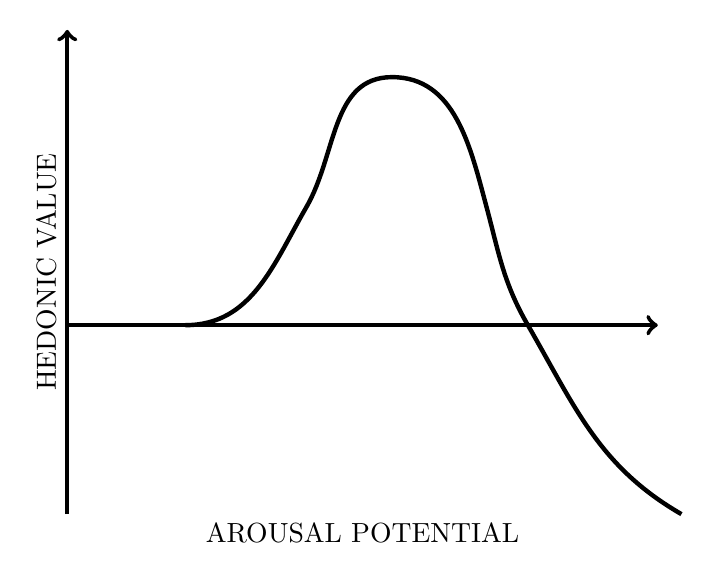
\begin{tikzpicture}[scale=0.75]
      % The image, for reference
      % \node[anchor=south west,inner sep=0] at (0,0) {\includegraphics[width=\textwidth]{wundt.png}};

      % Axes
      \draw[black,ultra thick,->] (1,0.8) -- (1,  9)   node[midway, above, sloped] {HEDONIC VALUE};     % y axis
      \draw[black,ultra thick,->] (1,4)   -- (11, 4);                                                   % x axis
      \path                       (1,0.8) -- (11, 0.8) node[midway, below]         {AROUSAL POTENTIAL}; % x axis label

      % Curve. The numbers come from tracing over wundt.png
      \draw[black,ultra thick] (3, 4)
           to[out=0,   in=240] (5.05, 6)
           to[out=60,  in=180] (6.5,  8.2)
           to[out=0,   in=105] (8.1,  6)
           to[out=-75, in=120] (8.8,  4)
           to[out=-60, in=150] (11.4, 0.8);

      % This version is closer, but a little jagged
      \iffalse
      \draw[black,ultra thick] (3, 4)
           to[out=0,   in=240] (5.05, 6)
           to[out=60,  in=225] (6,    8)
           to[out=45,  in=180] (6.5,  8.2)
           to[out=0,   in=135] (7.2,  8)
           to[out=-45, in=105] (8.1,  6)
           to[out=-75, in=120] (8.8,  4)
           to[out=-60, in=150] (11.4, 0.8);
      \fi
  \end{tikzpicture}

  \caption{The Wundt curve, reproduced from \citep{berlyne1970novelty}. The axes ``hedonic value'' and ``arousal potential'' are described as covering \textquote{reward value\dots preference or pleasure}, and \textquote{all the stimulus properties that tend to raise arousal, including novelty and complexity}, respectively.}

  \label{fig:wundt}
\end{figure}

\emph{Artificial curiosity} (AC) describes active learning systems which are rewarded based on how interesting the input or data they discover is \citep{schmidhuber2006developmental}. Although framed in the context of \emph{reinforcement learning}, this reliance on interest is clearly relevant to our theory exploration setting.

As an unsupervised learning task, AC has no access to labels or meanings associated with its input; the only features it can learn are the structure and relationships inherent in the data, in a similar way to our recurrent clustering algorithm. The unifying principle of AC methods is to force systems away from inputs which are not amenable to learning; either because they are so familiar that there is nothing left to learn, or so unfamiliar that they are unintelligible. The resulting behaviour is characterised by the \emph{Wundt curve} (shown in Figure \ref{fig:wundt}) \footnote{In practice, many measures avoid negative values for simplicity, in which cases we replace all negative points on the curve with zero.}, which has been used in psychology to explain human aesthetics and preferences \citep{berlyne1970novelty}. This same behaviour may be applicable to the theorems produced by a theory exploration system.

We can divide AC approaches into two groups: those which make \emph{explicit} use of interestingness, learning from signals which follow a Wundt curve; whilst \emph{implicit} approaches modify the \emph{output} of their learning algorithm(s), to engineer the overall system behaviour to follow a Wundt curve as an emergent property.

A framework encompassing many examples of the explicit approach is given in \citep{oudeyer2007intrinsic} in the context of reinforcement learning; for comparison, many similar measures are surveyed in a data mining context in \citep{geng2006interestingness}. Many more reinforcement learning examples can be found in \citep{Kaplan2006, Lipson2007, Luciw2011, Macedo2000, Ramik.Sabourin.Madani:2013, Roa.Kruijff.Jacobsson:2009, Schmidhuber:1991, oudeyer2004intelligent}; whilst more general descriptions are given in \citep{Schaul.Sun.Wierstra.ea:2011, Scott1989, maher2008achieving}, which may be more amenable to our theory exploration setting.

Many of these reward signals are based on information theory, with a prominent example being \emph{compression progress}: given a compressed representation of our previous observations, the ``progress'' is the space saved if we include the current observation. Observations which are incompressible or trivially compressible don't save any space, whilst observations which provide new insights into the structure of past experience can provide a space saving when compressed together. This seems particularly relevant for our problem of identifying interesting theorems: those new theorems (``observations'') which shorten the proofs of previously discovered theorems may be more general, more powerful and therefore more \emph{interesting} and hence worth keeping. In fact this is very similar to \qspec{}'s interestingness criterion.

Another example of explicit artificial curiosity is given in \citep{Hester.Stone:2012}, where world states which cause \emph{disagreement} among a population of decision trees (a \emph{random forest} \citep{randomforests}) are considered interesting. Since the models make stochastic predictions, the disagreement follows a Wundt curve as the complexity of state transitions increases: for parts of the state space which have been fully learned, the models will agree on accurate predictions; for parts which are unlearnable, the models cannot infer any structure, and will converge to reporting the same average value. Whilst the latter predictions may not be \emph{accurate}, they will be \emph{in agreement}, hence pushing down the interestingness of states which are too complex.

Many examples of the implicit case are based on \emph{coevolution}: rewarding one part of the system for exploiting another part, and vice versa. In \citep{Schmidhuber1999} a pair of learning algorithms place virtual ``bets'' on the outcome of actions, and the winner is rewarded at the expense of the loser. Due to the risk involved, each algorithm will only bet when it is confident in its prediction, and bets will only be actioned when each algorithm is confident in a \emph{different} outcome. The overall behaviour of this system is therefore similar to the explicit measure of disagreement used in the random forest example. In terms of theory exploration, such a scheme could be used to find theorems which are \emph{non-obvious}, and hence informative in some way to the user.

Another case is the ``darwinian brain'' of Fernando et al. \citep{fernando2013design1, fernando2013design2}. This coevolves a population of problem generators and problem solvers, rewarding the solvers based on their speed, and rewarding the generators based on the \emph{variance} of the solvers' speed. This avoids trivial problems (which all solvers can quickly overcome) and complex problems (which no solver can manage), and focuses on those with the most possibility for learning. It is easy to imagine such a general architecture being populated by conjecture generators and theorem provers to form a theory exploration system.

\paragraph{Evolutionary Computation} \leavevmode \newline

Coevolution is a form of \emph{evolutionary computation}; an umbrella term for heuristic search algorithms which mimic the process of evolution by natural selection among a population of candidate solutions \citep{back1997evolutionary}. Whilst \emph{genetic algorithms} are perhaps the most well-known instance of evolutionary computation, their use of \emph{strings} to represent solutions causes complications when comparing to a domain like theory exploration, where recursive structures of unbounded depth arise. Thankfully these problems are not insurmountable, for example \emph{genetic programming} can operate on tree-structures natively \citep{banzhaf1998genetic}, which makes evolutionary computation a useful source of ideas for reuse in our theory exploration setting (there are also precedents for using evolutionary computation in a theorem proving domain \citep{spector2008genetic}).

Traditionally, evolutionary approaches assign solutions a \emph{fitness} value, using a user-supplied \emph{fitness function}. Fitness should correlate with how well a solution solves the user's problem; for example, the fitness of a solution to some engineering problem may depend on the estimated materials cost. If we frame the task of theory exploration in evolutionary computation terms, the fitness function would be our interestingness measure.

Pure exploration (i.e. for its own sake) has been studied in evolutionary computation for two main reasons: \emph{artificial life} and \emph{deceptive problems}. The former attempts to gain insight into the nature of life and biology through competition over limited resources. Whilst this may have utility in resource allocation, e.g. efficient scheduling of a portfolio of ATP programs, there is no direct connection to interestingness in theory exploration, so we will not consider it further (note that similar resource-usage ideas can also be found in the literature on \emph{artificial economies}, e.g. \citep{baum2000evolution}).

On the other hand, work on deceptive problems is highly relevant, as it has lead to studying various notions of intrinsic fitness, which are analogous to the interestingness measures we want. Deceptive problems are those where \textquote{pursuing the objective may prevent the objective from being reached} \citep{lehman2011abandoning}, which is caused by the fitness (objective) function having many local optima which are easy to find (e.g. by hill climbing), but few global optima which are hard to find. Many approaches try to avoid deception by augmenting the given fitness function to promote \emph{diversity} and \emph{novelty}, such as \emph{niching methods} \citep{sareni1998fitness}.

One example is \emph{fitness sharing}, which divides up fitness values between identical or similar solutions. Say we have a user-provided fitness function $f$, and a population containing two identical solutions $s_1$ and $s_2$; hence $f(s_1) = f(s_2)$. In a fitness sharing scheme, we interpret fitness as a fixed resource, distributed according to $f$; when multiple individuals occupy the same point in the solution space, they must \emph{share} the fitness available there. We can describe the fitness \emph{allocated} to a solution by augmenting $f$, e.g. if we allocate fitness uniformly between identical solutions we get:

$$f'(x) = \frac{f(x)}{\sum_{i=1}^n \delta_{s_i x}}$$

Where $n$ is the population size, $s_i$ is the $i$th solution in the population and $\delta$ is the Kronecker delta function. In the example above, assuming there are no other copies in the population, then $f'(s_1) = \frac{f(s_1)}{2} = \frac{f(s_2)}{2} = f'(s_2)$. By sharing in this way, the fitness of each solution is balanced against redundancy in the population: there may still be many copies of a solution, but only when the fitness is high enough to justify all of them.

There are many variations on this theme, such as sharing between ``close'' solutions rather than just identical ones and judging distance based on fitness (AKA phenotypically) rather than based on the location in solution space (AKA genetically). Yet the underlying principle is always the same: penalise duplication in order to promote diversity. This lesson can be carried over to our theory exploration context, where a theorem should be considered less interesting if it is ``close'' to others which have been found.

In a similar way, we can bias our search procedure, rather than our fitness function, towards diversity. The search procedure in population-based evolutionary algorithms consists of \emph{selecting} one or more individuals from the population, e.g. via truncation (select the best $n$ individuals, discarding the rest); then \emph{transforming} the selected individuals, e.g. via mutation and crossover, to obtain new solutions.

Traditional selection methods are biased towards high fitness individuals (this is especially clear for truncation). Alternative schemes have been proposed which favour diversity \emph{at the expense of} fitness. For example, the fitness uniform selection scheme (FUSS) \citep{hutter2002fitness} selects a target fitness $f_t$ uniformly from the interval $\left[ f_{min}, f_{max} \right]$ between the highest and lowest of the population. An individual $s$ is then selected with fitness closest to $f_t$, i.e. $s = \argmin\limits_{x} \lvert f(x) - f_t \rvert$

In this way, the fitness function $f$ is used to assign comparable quantities to solutions, but it is not treated as the objective; instead, the implicit objective is to maintain a diverse population, with individuals spread out uniformly in fitness space. This approach seems useful for informing our work in theory exploration, as it supports search criteria which \emph{describe} solutions, but which we may not want to \emph{optimise}. As a simple example, we might distinguish different forms of theorem by measuring how balanced their syntax trees are (-1 for left-leaning, +1 for right leaning, 0 for balanced); but it would be senseless to \emph{maximise} how far they lean.

Once we begin this process of augmenting fitness functions, or abandoning their use as objectives, an obvious question arises: what happens if our new function contains nothing of the original? This kind of pure exploration scenario leads to a variety of ideas for \emph{instrinsic} fitness, such as novelty \citep{lehman2011abandoning}, which can lead to learning useful ``stepping stones'' even in objective-driven domains. Such intrinsic notions of fitness are direct analogues of the interestingness measures we seek for theory exploration.
